% Project plan for the loading update of PoliVerse. Numbers come from plan.py.
\documentclass[plan]{se2doc}
% Written once per project; every document reads it.
% Each document sets its own \docversion and \revision lines after reading this.
\project{PoliVerse Loading Update}
\authors{Samuele Segrini}
\docdate{10 November 2026}

\docversion{0.1}
\revision{0.1}{10 Nov 2026}{First plan, from RASD 1.0 and DD 0.1}
\usepackage{float}
\newcommand\planbac{339}
\newcommand\planleft{319.1}
\newcommand\plancritical{D1, D2, M1.1, M1.2, M1.3, M1.5, M2.1, M2.2, M2.3, M2.4, M2.6, M7.3, M7.4, M8.1, M8.3, M8.4, A1, A2}
\newcommand\plancriticalhours{162}
\newcommand\planend{25 June 2027}
\newcommand\planstart{16 November 2026}


\begin{document}
\maketitle

% DRAFT, rewrite
\section{Scope and success criteria}
The plan covers the loading update specified in the RASD and designed in the DD:
eight milestones of implementation, the documents, and an acceptance test on the
phone. One developer works on it part time.

The update succeeds when:
\begin{itemize}
  \item every requirement R1 to R40 has a passing test that carries its id;
  \item the performance requirements P1 to P9 hold on the iPhone 12 Pro, read from the loading ledger against the baseline of milestone M1;
  \item the six use cases pass when played by hand with a real account.
\end{itemize}

\section{Estimate}
\subsection{Function points}
The functions are counted from the RASD's use cases and data. Weights are the IFPUG
defaults (ILF 7/10/15, EIF 5/7/10, EI 3/4/6, EO 4/5/7, EQ 3/4/6).
% TODO: check weights and COCOMO constants against the slides of lecture 06.
\begin{longtable}{@{}p{0.45\linewidth} l r r l r@{}}
\toprule Function & Type & DET & RET/FTR & Complexity & FP \\ \midrule
Stored parts with fetch time and account & ILF & 6 & 2 & low & 7 \\
Loading ledger entries & ILF & 9 & 2 & low & 7 \\
New marks & ILF & 3 & 1 & low & 7 \\
Offline pack state & ILF & 5 & 1 & low & 7 \\
Speculative budget settings and daily count & ILF & 5 & 1 & low & 7 \\
Career data of the Politecnico & EIF & 20 & 6 & average & 7 \\
Room bookings of the Politecnico & EIF & 6 & 1 & low & 5 \\
Timetable of the Politecnico & EIF & 10 & 1 & low & 5 \\
Course pages and syllabi & EIF & 12 & 2 & low & 5 \\
Retry a failed section & EI & 2 & 1 & low & 3 \\
Switch the offline pack on or off and start it & EI & 3 & 1 & low & 3 \\
Allow speculative requests on cellular & EI & 2 & 1 & low & 3 \\
Enable kinds of change notification and the haptic & EI & 5 & 1 & low & 3 \\
Sign out (delete copies marks and ledger) & EI & 1 & 3 & low & 3 \\
Screen shown part by part with section states & EO & 8 & 3 & average & 5 \\
Free rooms in relevance order with boundary updates & EO & 7 & 3 & average & 5 \\
Changed items marked and notified & EO & 6 & 2 & low & 4 \\
Loading report with medians and percentiles & EO & 9 & 1 & low & 4 \\
Offline pack status & EQ & 5 & 1 & low & 3 \\
Stored copy shown with its age & EQ & 4 & 1 & low & 3 \\
Prefetched part shown without a request & EQ & 3 & 2 & low & 3 \\
\midrule \multicolumn{5}{@{}l}{Unadjusted function points} & 99 \\
\bottomrule
\end{longtable}


\subsection{Size and effort}
\begin{center}
\begin{tabular}{@{}l r@{}}
\toprule
Unadjusted function points & 99 \\
Size at 53 lines per function point & 5.25 KSLOC \\
COCOMO II exponent ($B + 0.01 \sum SF$, nominal) & 1.0997 \\
Effort ($A \cdot \mathrm{KSLOC}^E$, $A = 2.94$, multipliers nominal) & 18.2 person-months \\
Effort at 152 hours per person-month & 2766 hours \\
\bottomrule
\end{tabular}
\end{center}

Assumptions:
\begin{itemize}
  \item 53 lines per function point: the usual backfiring figure for Java-like languages. No published figure exists for Swift.
  \item COCOMO II post-architecture, all scale factors and effort multipliers nominal.
\end{itemize}
The result is far above the bottom-up total of \planbac{} hours in the next
section. That is expected: the model is calibrated on teams building a product
from nothing, with all its overheads, while this update extends a store layer that
exists and is done by one person who knows it. The estimate is kept as an upper
bound and as a number to compare with the hours actually logged. The schedule
uses the bottom-up figures.

\section{WBS and schedule}
\subsection{Work breakdown}
Leaves are 3 to 16 hours. Float and the critical path come from the dependencies
alone, as if tasks could run in parallel.
\begin{longtable}{@{}l p{0.42\linewidth} r p{0.16\linewidth} r l@{}}
\toprule Id & Task & Hours & Depends on & Float & Critical \\
\endhead
\midrule \textbf{D} & \textbf{Documents} & \textbf{23} & & & \\
D1 & RASD & 8 &  & 0 & yes \\
D2 & Design document & 8 & D1 & 0 & yes \\
D3 & Alloy model and its check & 4 & D1 & 150 &  \\
D4 & Project plan & 3 & D1 & 151 &  \\
\midrule \textbf{M1} & \textbf{Loading ledger} & \textbf{30} & & & \\
M1.1 & RequestGate as recording pass-through & 8 & D2 & 0 & yes \\
M1.2 & LoadingLedger and its file & 8 & M1.1 & 0 & yes \\
M1.3 & Report in diagnostics & 6 & M1.2 & 0 & yes \\
M1.4 & Screen tokens on the main screens & 4 & M1.2 & 2 &  \\
M1.5 & Baseline run on the iPhone 12 Pro & 4 & M1.3 M1.4 & 0 & yes \\
\midrule \textbf{M2} & \textbf{Parts} & \textbf{54} & & & \\
M2.1 & Part type and Progress on Resource & 8 & M1.5 & 0 & yes \\
M2.2 & Loader per part and PartStore & 16 & M2.1 & 0 & yes \\
M2.3 & Query phases & 8 & M2.2 & 0 & yes \\
M2.4 & Career as first user & 8 & M2.3 & 0 & yes \\
M2.5 & Search sources in parallel & 4 & M1.5 & 116 &  \\
M2.6 & Integration tests with scripted transport & 10 & M2.4 & 0 & yes \\
\midrule \textbf{M3} & \textbf{Section kit} & \textbf{48} & & & \\
M3.1 & arriving modifier and SectionStatus & 10 & M2.3 & 12 &  \\
M3.2 & RevealRenderer & 12 & M3.1 & 12 &  \\
M3.3 & ShapeMemory & 4 & M3.1 & 28 &  \\
M3.4 & Carriera Appelli Libretto & 8 & M3.2 M2.6 & 12 &  \\
M3.5 & Oggi & 6 & M3.2 & 14 &  \\
M3.6 & UI tests and hitch measurement & 8 & M3.3 M3.4 M3.5 & 12 &  \\
\midrule \textbf{M4} & \textbf{Rooms} & \textbf{32} & & & \\
M4.1 & RelevanceOrder & 4 & M1.5 & 74 &  \\
M4.2 & Rooms assigned per batch and stable list & 8 & M4.1 M3.1 & 36 &  \\
M4.3 & Map colours as rooms arrive & 6 & M4.2 & 38 &  \\
M4.4 & BoundaryClock & 8 & M4.2 & 36 &  \\
M4.5 & Tests and first-room measurement & 6 & M4.3 M4.4 & 36 &  \\
\midrule \textbf{M5} & \textbf{Slow parts} & \textbf{22} & & & \\
M5.1 & DeadlinePolicy in the loader & 8 & M2.6 & 36 &  \\
M5.2 & Host breaker in RequestGate & 8 & M1.5 & 86 &  \\
M5.3 & Tests with a transport that never answers & 6 & M5.1 M5.2 & 36 &  \\
\midrule \textbf{M6} & \textbf{Changes} & \textbf{34} & & & \\
M6.1 & ChangeDetector and changes on Query & 10 & M2.6 & 24 &  \\
M6.2 & NewMarks and the mark in the section kit & 8 & M6.1 M3.6 & 16 &  \\
M6.3 & UpdateFeed as consumer and new notification kinds & 10 & M6.1 & 24 &  \\
M6.4 & Tests with fixtures & 6 & M6.2 M6.3 & 16 &  \\
\midrule \textbf{M7} & \textbf{Prefetch} & \textbf{36} & & & \\
M7.1 & SpeculativeBudget and its settings page & 10 & M1.5 & 32 &  \\
M7.2 & Lanes in RequestGate & 8 & M7.1 & 32 &  \\
M7.3 & TimetablePrefetch and its two triggers & 10 & M7.2 M2.6 & 0 & yes \\
M7.4 & Tests and hit-rate check & 8 & M7.3 & 0 & yes \\
\midrule \textbf{M8} & \textbf{Offline} & \textbf{40} & & & \\
M8.1 & OfflinePack and the processing task & 14 & M7.4 & 0 & yes \\
M8.2 & Offline page in Impostazioni & 8 & M8.1 & 2 &  \\
M8.3 & Behaviour with no connection on every pack screen & 10 & M8.1 M3.6 & 0 & yes \\
M8.4 & Tests and storage measurement & 8 & M8.2 M8.3 & 0 & yes \\
\midrule \textbf{A} & \textbf{Acceptance} & \textbf{20} & & & \\
A1 & Use cases played on the phone & 8 & M4.5 M5.3 M6.4 M8.4 & 0 & yes \\
A2 & Fixes from acceptance & 12 & A1 & 0 & yes \\
\midrule & \textbf{Budget at completion} & \textbf{339} & & & \\
\bottomrule
\end{longtable}


\noindent Critical path (\plancriticalhours{} hours): \plancritical.

\subsection{Schedule}
With one developer the tasks run one after another, milestone after milestone.
The schedule assumes 10 hours a week, as 2 hours on each working day, from
\planstart. \planleft{} hours remain, and the planned end is \planend.

\begin{figure}[H]
\centering
\begin{ganttchart}[
  time slot format=isodate, x unit=0.047cm, y unit chart=0.36cm, y unit title=0.45cm,
  title label font=\scriptsize, bar label font=\scriptsize, group label font=\scriptsize\bfseries,
  milestone label font=\scriptsize\itshape, bar height=0.6, group height=0.25,
  milestone height=0.6, vgrid={*6{draw=none}, dotted}, hgrid=false
  ]{2026-11-01}{2027-06-30}
\gantttitlecalendar{year, month=shortname} \\
\ganttgroup{D Documents}{2026-11-16}{2026-11-17} \\
\ganttbar[bar/.append style={fill=gray!85}]{D2}{2026-11-16}{2026-11-16} \\
\ganttbar{D3}{2026-11-16}{2026-11-17} \\
\ganttbar{D4}{2026-11-17}{2026-11-17} \\
\ganttgroup{M1 Loading ledger}{2026-11-17}{2026-12-08} \\
\ganttbar[bar/.append style={fill=gray!85}]{M1.1}{2026-11-17}{2026-11-23} \\
\ganttbar[bar/.append style={fill=gray!85}]{M1.2}{2026-11-23}{2026-11-27} \\
\ganttbar[bar/.append style={fill=gray!85}]{M1.3}{2026-11-27}{2026-12-02} \\
\ganttbar{M1.4}{2026-12-02}{2026-12-04} \\
\ganttbar[bar/.append style={fill=gray!85}]{M1.5}{2026-12-04}{2026-12-08} \\
\ganttmilestone{M1 done}{2026-12-08} \\
\ganttgroup{M2 Parts}{2026-12-08}{2027-01-14} \\
\ganttbar[bar/.append style={fill=gray!85}]{M2.1}{2026-12-08}{2026-12-14} \\
\ganttbar[bar/.append style={fill=gray!85}]{M2.2}{2026-12-14}{2026-12-24} \\
\ganttbar[bar/.append style={fill=gray!85}]{M2.3}{2026-12-24}{2026-12-30} \\
\ganttbar[bar/.append style={fill=gray!85}]{M2.4}{2026-12-30}{2027-01-05} \\
\ganttbar{M2.5}{2027-01-05}{2027-01-07} \\
\ganttbar[bar/.append style={fill=gray!85}]{M2.6}{2027-01-07}{2027-01-14} \\
\ganttmilestone{M2 done}{2027-01-14} \\
\ganttgroup{M3 Section kit}{2027-01-14}{2027-02-17} \\
\ganttbar{M3.1}{2027-01-14}{2027-01-21} \\
\ganttbar{M3.2}{2027-01-21}{2027-01-29} \\
\ganttbar{M3.3}{2027-01-29}{2027-02-02} \\
\ganttbar{M3.4}{2027-02-02}{2027-02-08} \\
\ganttbar{M3.5}{2027-02-08}{2027-02-11} \\
\ganttbar{M3.6}{2027-02-11}{2027-02-17} \\
\ganttmilestone{M3 done}{2027-02-17} \\
\ganttgroup{M4 Rooms}{2027-02-17}{2027-03-11} \\
\ganttbar{M4.1}{2027-02-17}{2027-02-19} \\
\ganttbar{M4.2}{2027-02-19}{2027-02-25} \\
\ganttbar{M4.3}{2027-02-25}{2027-03-02} \\
\ganttbar{M4.4}{2027-03-02}{2027-03-08} \\
\ganttbar{M4.5}{2027-03-08}{2027-03-11} \\
\ganttmilestone{M4 done}{2027-03-11} \\
\ganttgroup{M5 Slow parts}{2027-03-11}{2027-03-26} \\
\ganttbar{M5.1}{2027-03-11}{2027-03-17} \\
\ganttbar{M5.2}{2027-03-17}{2027-03-23} \\
\ganttbar{M5.3}{2027-03-23}{2027-03-26} \\
\ganttmilestone{M5 done}{2027-03-26} \\
\ganttgroup{M6 Changes}{2027-03-26}{2027-04-20} \\
\ganttbar{M6.1}{2027-03-26}{2027-04-02} \\
\ganttbar{M6.2}{2027-04-02}{2027-04-08} \\
\ganttbar{M6.3}{2027-04-08}{2027-04-15} \\
\ganttbar{M6.4}{2027-04-15}{2027-04-20} \\
\ganttmilestone{M6 done}{2027-04-20} \\
\ganttgroup{M7 Prefetch}{2027-04-20}{2027-05-14} \\
\ganttbar{M7.1}{2027-04-20}{2027-04-27} \\
\ganttbar{M7.2}{2027-04-27}{2027-05-03} \\
\ganttbar[bar/.append style={fill=gray!85}]{M7.3}{2027-05-03}{2027-05-10} \\
\ganttbar[bar/.append style={fill=gray!85}]{M7.4}{2027-05-10}{2027-05-14} \\
\ganttmilestone{M7 done}{2027-05-14} \\
\ganttgroup{M8 Offline}{2027-05-14}{2027-06-11} \\
\ganttbar[bar/.append style={fill=gray!85}]{M8.1}{2027-05-14}{2027-05-25} \\
\ganttbar{M8.2}{2027-05-25}{2027-05-31} \\
\ganttbar[bar/.append style={fill=gray!85}]{M8.3}{2027-05-31}{2027-06-07} \\
\ganttbar[bar/.append style={fill=gray!85}]{M8.4}{2027-06-07}{2027-06-11} \\
\ganttmilestone{M8 done}{2027-06-11} \\
\ganttgroup{A Acceptance}{2027-06-11}{2027-06-25} \\
\ganttbar[bar/.append style={fill=gray!85}]{A1}{2027-06-11}{2027-06-17} \\
\ganttbar[bar/.append style={fill=gray!85}]{A2}{2027-06-17}{2027-06-25} \\
\ganttmilestone{A done}{2027-06-25}
\end{ganttchart}

\caption{Schedule. Dark bars are on the critical path; diamonds close a milestone.}
\end{figure}

\begin{center}\small
\begin{tabularx}{\linewidth}{@{}l l X@{}}
\toprule Milestone & Planned date & Closed by \\ \midrule
M1 Loading ledger & 2026-12-08 & Baseline run on the iPhone 12 Pro \\
M2 Parts & 2027-01-14 & Integration tests with scripted transport \\
M3 Section kit & 2027-02-17 & UI tests and hitch measurement \\
M4 Rooms & 2027-03-11 & Tests and first-room measurement \\
M5 Slow parts & 2027-03-26 & Tests with a transport that never answers \\
M6 Changes & 2027-04-20 & Tests with fixtures \\
M7 Prefetch & 2027-05-14 & Tests and hit-rate check \\
M8 Offline & 2027-06-11 & Tests and storage measurement \\
A Acceptance & 2027-06-25 & Fixes from acceptance \\
\bottomrule
\end{tabularx}
\end{center}


\section{Risk management}
Likelihood and impact are on a scale of 1 to 5.
{\small
\begin{longtable}{@{}l p{0.27\linewidth} l r r r p{0.33\linewidth}@{}}
\toprule Id & Risk & Category & L & I & L$\times$I & Mitigation \\ \midrule
\endhead
K4 & The Politecnico changes or blocks an endpoint as happened before & business & 3 & 5 & 15 & No new endpoint; daily limit on speculative requests; stored copies keep screens usable \\
K1 & The new fetch signature breaks the 19 existing resources or their tests & technical & 3 & 4 & 12 & Default implementation forwards to the old signature; migrate one resource (career) first \\
K3 & iOS rarely runs the background tasks so prefetch and the pack seldom happen & technical & 4 & 3 & 12 & Also run the prefetch after every foreground pass; show pack state and a manual start \\
K5 & Change detection reports changes that are not real and notifies wrongly & technical & 3 & 4 & 12 & Compare by identity only for kinds with stable ids; reuse the exam policy and its daily limit; fixtures from real payloads \\
K8 & The estimate is too low for one developer working part time & project & 4 & 3 & 12 & Milestones ship one by one; M4 to M8 can be dropped or reordered without breaking earlier ones; earned value at each milestone \\
K2 & The reveal causes hitches on the iPhone 12 Pro & technical & 3 & 3 & 9 & Measure P6 in M3 before applying it to more screens; fall back to a cross-fade per section \\
K9 & Scope grows with new ideas during the build & project & 3 & 3 & 9 & New ideas go to the RASD as a new revision first; habit prediction stays out of scope \\
K6 & Room bookings change during the day more often than assumed (D6) & technical & 2 & 3 & 6 & Boundary refresh re-requests rooms on screen; show the age of the bookings \\
K7 & Stored parts and the offline pack grow beyond the storage limit & technical & 2 & 3 & 6 & Measure in M8 against P9; one campus only; delete parts of past weeks \\
K10 & Deadline and breaker values hide answers that would have come & technical & 2 & 2 & 4 & Initial values confirmed with the ledger baseline before M5 ships \\
\bottomrule
\end{longtable}}

\begin{figure}[H]
\centering
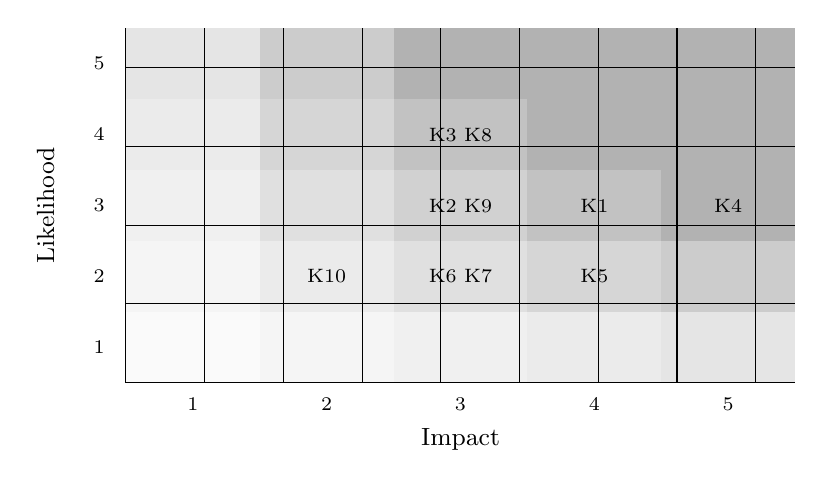
\begin{tikzpicture}[x=1.7cm, y=0.9cm]
\fill[gray!4] (0,0) rectangle (1,1);
\fill[gray!8] (1,0) rectangle (2,1);
\fill[gray!12] (2,0) rectangle (3,1);
\fill[gray!16] (3,0) rectangle (4,1);
\fill[gray!20] (4,0) rectangle (5,1);
\fill[gray!8] (0,1) rectangle (1,2);
\fill[gray!16] (1,1) rectangle (2,2);
\node[font=\scriptsize] at (1.5,1.5) {K10};
\fill[gray!24] (2,1) rectangle (3,2);
\node[font=\scriptsize] at (2.5,1.5) {K6 K7};
\fill[gray!32] (3,1) rectangle (4,2);
\node[font=\scriptsize] at (3.5,1.5) {K5};
\fill[gray!40] (4,1) rectangle (5,2);
\fill[gray!12] (0,2) rectangle (1,3);
\fill[gray!24] (1,2) rectangle (2,3);
\fill[gray!36] (2,2) rectangle (3,3);
\node[font=\scriptsize] at (2.5,2.5) {K2 K9};
\fill[gray!48] (3,2) rectangle (4,3);
\node[font=\scriptsize] at (3.5,2.5) {K1};
\fill[gray!60] (4,2) rectangle (5,3);
\node[font=\scriptsize] at (4.5,2.5) {K4};
\fill[gray!16] (0,3) rectangle (1,4);
\fill[gray!32] (1,3) rectangle (2,4);
\fill[gray!48] (2,3) rectangle (3,4);
\node[font=\scriptsize] at (2.5,3.5) {K3 K8};
\fill[gray!60] (3,3) rectangle (4,4);
\fill[gray!60] (4,3) rectangle (5,4);
\fill[gray!20] (0,4) rectangle (1,5);
\fill[gray!40] (1,4) rectangle (2,5);
\fill[gray!60] (2,4) rectangle (3,5);
\fill[gray!60] (3,4) rectangle (4,5);
\fill[gray!60] (4,4) rectangle (5,5);
\draw (0,0) grid (5,5);
\foreach \n in {1,...,5} {
  \node[font=\scriptsize] at (\n-0.5,-0.3) {\n};
  \node[font=\scriptsize] at (-0.2,\n-0.5) {\n};
}
\node[font=\small] at (2.5,-0.8) {Impact};
\node[font=\small, rotate=90] at (-0.6,2.5) {Likelihood};
\end{tikzpicture}

\caption{Open risks by likelihood and impact.}
\end{figure}
% TODO: redraw the plot the way lecture 06 draws it once the slide is at hand.

\section{Monitoring}
Hours are logged in \texttt{data/hours.csv} and progress in the
\texttt{percent\_complete} column of \texttt{data/wbs.csv}. At the end of each
milestone the earned value is computed (planned value, earned value, actual cost,
their variances and indices, and the estimate at completion) and a row is added to
\texttt{data/ev.csv}. No hours have been logged yet, so there is no row.

\section{Hours per task}
% TODO: \effort{task}{hours} per task from data/hours.csv, then \printeffort.
To be recorded as the work proceeds.

\end{document}
